\section{Orchestration}

Modern orchestration and containerization techniques have been rapidly evolving for the last decade.
To avoid issues due to different environments and dependencies, containers arose as a lightweight alternative to heavier virtual machines.
The most popular containerization software, Docker, was released in 2013.
Multiple individual containers quickly got grouped together to separate concerns and allow decoupled workloads.
These container groups became especially useful and popular with the rise of micro-service architectures.
Handling various containers at the same time is challenging.
Techniques such as Docker Compose made this easier.
However, dynamically scaling and handling failing containers was still difficult.
These dynamic swarms of containers needed additional management tooling for orchestration.
Kubernetes, the most prominent orchestrator to date, was released in 2014.
Since then many new endevours formed to unify and streamline future developents in the field.
Examples include the Open Container Initiative \cite{open_container_initiative} or the Moby Project \cite{moby_project}.
Many different alternatives and competitors to Docker and Kubernetes have developed over the years.

\subsection{ML Containerization \& Orchestration}

Performing ML in containers is an effective approach.
FLOps aims to automate and orchestrate FL workloads on distributed heterogeneous machines.
It is crucial to confirm that doing FL/ML via orchestrated containers is viable.
In addition, FL processes should not suffer from bottlenecks and problems due to running inside containers.
In 2017, Xu et al. \cite{paper:dl_via_docker} evaluated deep learning (DL) tool performance in docker containers.
They analyzed CPU, GPU, and I/O utilizations.
They found that DL works equally well in containers as running it directly on the host machines.

Containerized ML is widely used today.
In 2022, Openja et al. \cite{paper:ml_practices_on_docker} analyzed more than 400 different open-source ML-based projects that use docker containers.
These projects used containers for various tasks.
A popular application of containerization technologies in ML is to streamline and improve deployment efforts.
This work demonstrates that containers are used in all ML-related tasks nowadays.

Orchestration efforts are optional for classic ML but essential for FL.
As discussed in \ref{section:federated_learning}, classic centralized ML can be trained on a single powerful machine.
FL, especially Cross-Device edge FL, can involve massive dynamic numbers of devices.
Managing all these components is challenging.
Training an ML model requires more than just the ML code and model.
The device performing the training needs to support the necessary environment and dependency requirements.
The setup and configuration of devices is a limiting and error-prone task.
To avoid potential issues and to allow as many devices to participate as possible, FL should use containers. 


\subsection{Oakestra}

FLOps primarily focuses on enabling practical FL on real machines.
The main target group for cross-device FL is heterogeneous edge devices.
Kubernetes is not designed for the edge but for homogeneous, resource-rich cloud environments, whereas Oakestra is designed for the edge and outperforms Kubernetes there \cite{paper:oakestra_usenix}.

Oakestra is a hierarchical, open-source orchestrator for edge computing.
It has a lightweight and flexible code base.
It features many novel techniques, such as semantic overlay networking for efficient service communication.

\begin{figure}[!ht]
    % \begin{adjustwidth}{-\oddsidemargin-1in}{-\rightmargin}
    \begin{adjustwidth}{-0.1\paperwidth}{-0.1\paperwidth}
        \centering
        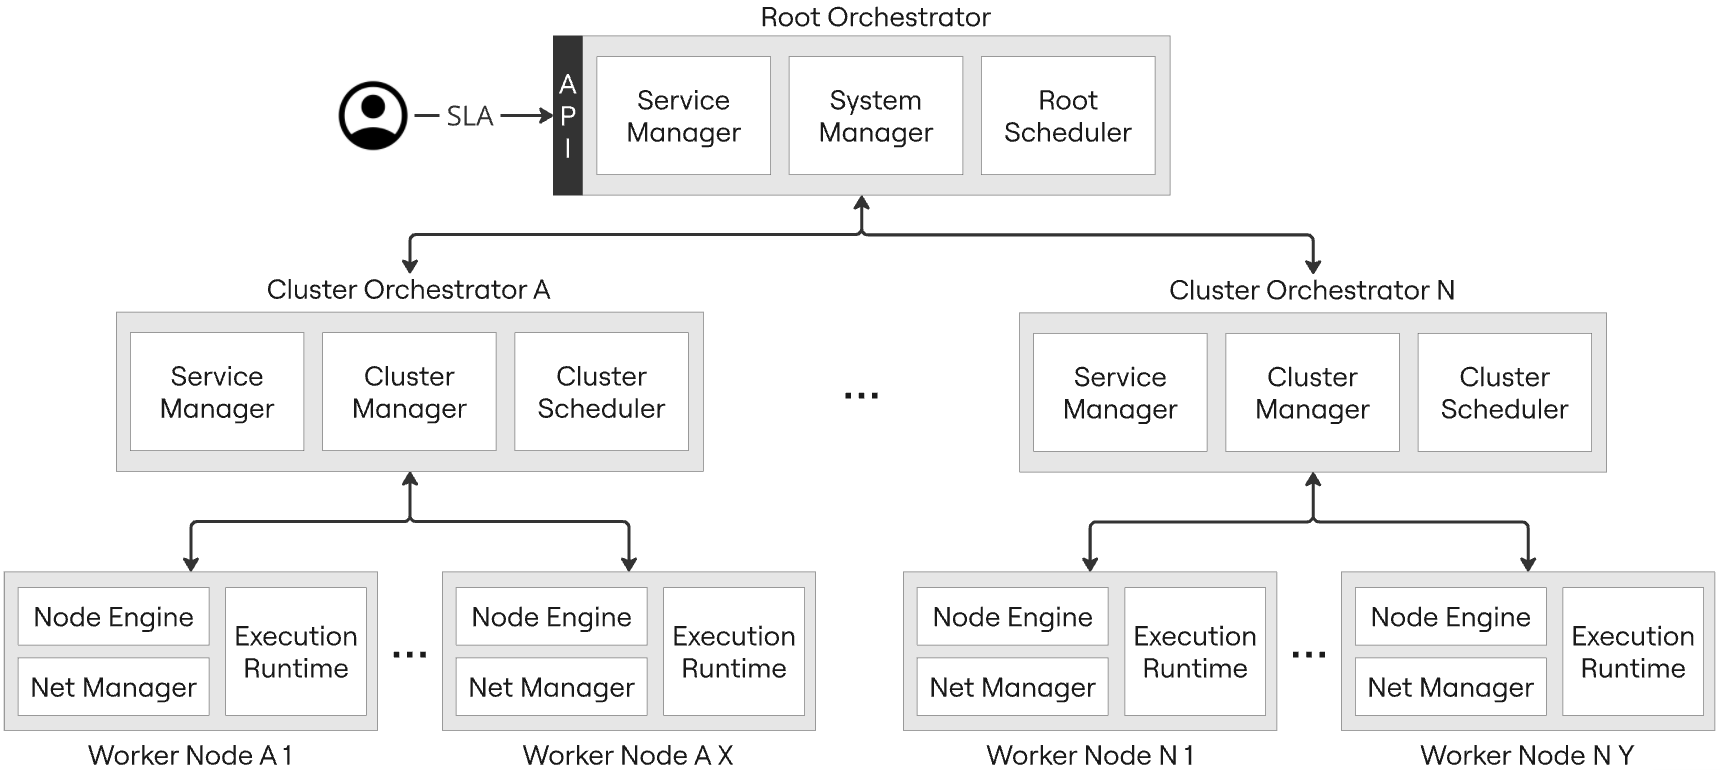
\includegraphics[width=0.9\paperwidth]{oakestra_simple_architecture.png}
        \caption{Simplified Oakestra Architecture}
        \label{fig:simple_oakestra_architecture}
    \end{adjustwidth}
\end{figure}

Figure \ref{fig:simple_oakestra_architecture} shows a simplified architecture of Oakestra.
This unique federated three-tiered structure allows for scalable delegate task scheduling and execution.
Instead of a single control plane, as in Kubernetes, Oakestra distributes its control among the root and cluster orchestrators.
Oakestra specializes in handling resource-constrained, heterogeneous devices that are spread across various geographical areas.
Different infrastructure providers can have their own isolated cluster and cluster orchestrator.
Cluster orchestrators can only access detailed information about workers from their own cluster.
The metrics they share with the root are distilled and no longer contain sensitive individual metadata.
This is an ideal environment for FL because this layout supports privacy on a structural level.
FLOps uses Oakestra to orchestrate its components.

\pagebreak
